\documentclass[10pt,openright,twoside,french]{book}

\usepackage{marvosym}
\input philippe2013
\input philippe2013_activites

\pagestyle{empty}

\begin{document}

\TitreExo{\bsc{iii} - 1}{Statistiques}
\exo On a relevé les notes annuelles de mathématiques et de français dans une classe de première \bsc{s.t.m.g.}\par
On a dessiné deux diagrammes en boîtes associés à ces notes : celui du haut pour les mathématiques et celui du bas pour le français.

\begin{center}
    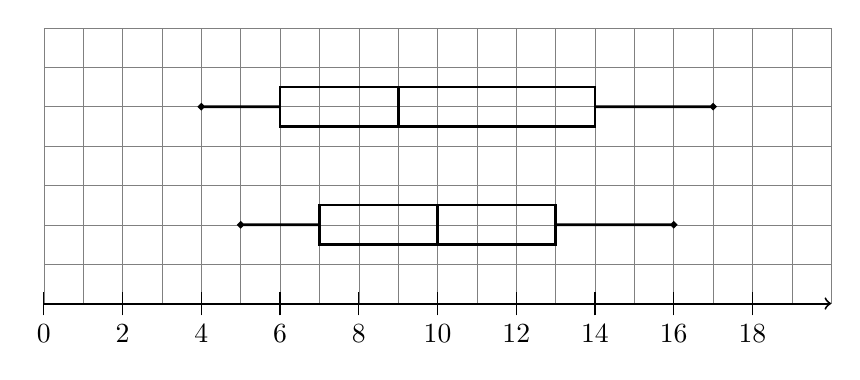
\begin{tikzpicture}
        \draw[help lines] (0,0) grid[step=5mm] (10,3.5);
        \draw[->,line width=0.7pt] (0,0) -- (10,0);
        \foreach \x in {0,2,...,19} \draw (\x/2,-0.15)node[below] {\x} -- (\x/2,0.15);
% diagramme en boîte 1 :
        \def\y{2.5}\def\mini{4}\def\qA{6}\def\med{9}\def\qB{14}\def\maxi{17}
        \draw[line width=1pt] (\mini/2,\y) circle (0.7pt) -- (\mini/2,\y) -- (\qA/2,\y);
        \draw[line width=1pt] (\qA/2,\y-0.25) rectangle (\qB/2,\y+0.25);
        \draw[line width=1pt] (\qB/2,\y) -- (\maxi/2,\y) -- (\maxi/2,\y) circle (0.7pt);
        \draw[line width=1pt] (\med/2,\y-0.25)--(\med/2,\y+0.25);
% diagramme en boîte 2 :
        \def\y{1}
        \def\mini{5}\def\maxi{16}
        \def\qA{7}\def\med{10}\def\qB{13}
        \draw[line width=1pt] (\mini/2,\y) circle (0.7pt)--(\mini/2,\y) -- (\qA/2,\y);
        \draw[line width=1pt] (\qA/2,\y-0.25) rectangle (\qB/2,\y+0.25);
        \draw[line width=1pt] (\qB/2,\y) -- (\maxi/2,\y)--(\maxi/2,\y) circle (0.7pt);
        \draw[line width=1pt] (\med/2,\y-0.25)--(\med/2,\y+0.25);
    \end{tikzpicture}
\end{center}

\begin{enumerate}
    \item Donner pour chaque série de notes :
    \begin{enumerate}
        \item l'étendue $E$ ;
        \item la médiane $M_e$ ;
        \item les quartiles et l'écart interquartile.
    \end{enumerate}
    \item Compléter les phrases suivantes :
    \begin{enumerate}
        \item En mathématiques, au plus \ldots\ldots \% des élèves ont une note supérieure à $14$.
        \item En français, au moins \ldots\ldots \% des élèves ont une note comprise entre $7$ et $13$.
        \item En mathématiques, au moins $25\%$ des élèves ont une note inférieure à \ldots
        \item En français, au moins $50\%$ des élèves ont une note inférieure à \ldots
    \end{enumerate}
    \item Dans quelle matière les notes sont-elles plus dispersées ? Donner deux critères.
\end{enumerate}\[*\]

\exo $\np{1000}$ personnes de différents laboratoires ont mesuré la densité d'un produit :
\begin{center}
    \begin{tabular}{|c|*{12}{>{\centering\arraybackslash}m{7mm}|}}
        \hline
            Densité & 8 & 8,1 & 8,2 & 8,3 & 8,4 & 8,5 & 8,6 & 8,7 & 8,8 & 8,9 & 9 & 9,1 \\
        \hline
            Effectifs & 4 & 20 & 43 & 100 & 200 & 250 & 190 & 115 & 50 & 19 & 6 & 3 \\
        \hline
    \end{tabular}
\end{center}

On arrondira les résultats au \textbf{dixième} près.

\begin{enumerate}
    \item En utilisant la fonction {\tt Stats} de la calculatrice, déterminer pour cette série statistique la moyenne $\overline x$, $\mtc Q_1$, la médiane $M_e$, $\mtc Q_3$ et l'écart-type $\sigma$.
    \item Construire le diagramme en boîte de cette série statistique.
    \item Déterminer l'intervalle $I_1 = \intervalleff{\overline x - \sigma}{\overline x + \sigma}$.
    \item Quel est le pourcentage de résultats qui appartiennent à $I_1$ ?
    \item Déterminer l'intervalle $I_2 = \intervalleff{\overline x - 2\sigma}{\overline x + 2\sigma}$.
    \item Quel est le pourcentage de résultats qui appartiennent à $I_2$ ?
\end{enumerate}
\end{document} 